\section{eo\-Pareto\-Sharing$<$ EOT, worth\-T $>$ Class Template Reference}
\label{classeoParetoSharing}\index{eoParetoSharing@{eoParetoSharing}}
Inheritance diagram for eo\-Pareto\-Sharing$<$ EOT, worth\-T $>$::\begin{figure}[H]
\begin{center}
\leavevmode
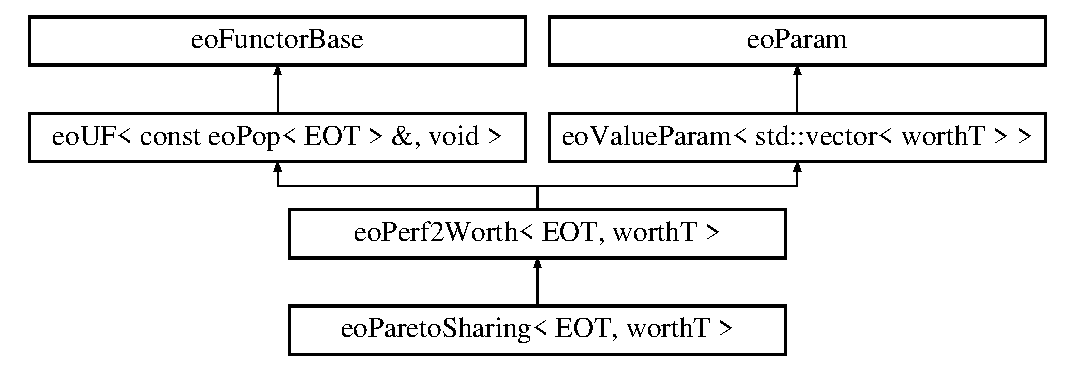
\includegraphics[height=4cm]{classeoParetoSharing}
\end{center}
\end{figure}
\subsection*{Public Member Functions}
\begin{CompactItemize}
\item 
{\bf eo\-Pareto\-Sharing} (double \_\-niche\-Size)\label{classeoParetoSharing_99666671930abc479a2f5e5dd2914d41}

\item 
{\bf eo\-Pareto\-Sharing} (double \_\-niche\-Size, {\bf eo\-Pareto\-Phen\-Dist}$<$ EOT, worth\-T $>$ \&\_\-dist)\label{classeoParetoSharing_5ad0d5b6a1c1f4fc17bb9a319f18d645}

\item 
void {\bf operator} ()(const {\bf eo\-Pop}$<$ EOT $>$ \&\_\-pop)\label{classeoParetoSharing_df55496bf711d4614bcf42d157a4b4de}

\end{CompactItemize}
\subsection*{Private Member Functions}
\begin{CompactItemize}
\item 
double {\bf sh} (double {\bf dist}, double {\bf Dmax})\label{classeoParetoSharing_ce18ecb042033d564be6379869f2be88}

\end{CompactItemize}
\subsection*{Private Attributes}
\begin{CompactItemize}
\item 
double {\bf niche\-Size}\label{classeoParetoSharing_0da31e076cf2098639cd1a9fa06f3942}

\item 
{\bf eo\-Pareto\-Phen\-Dist}$<$ EOT, worth\-T $>$ \& {\bf dist}\label{classeoParetoSharing_f5cff5bf666314e59d58043531253b1b}

\item 
{\bf eo\-Pareto\-Euclid\-Dist}$<$ EOT $>$ {\bf euc\_\-dist}\label{classeoParetoSharing_9b8e6e2c76d816afb23dfdbf91dabf57}

\item 
double {\bf Dmax}\label{classeoParetoSharing_35449ebac125955c49a6d34db0e710b3}

\end{CompactItemize}
\subsection*{Classes}
\begin{CompactItemize}
\item 
class {\bf d\-Matrix}
\end{CompactItemize}


\subsection{Detailed Description}
\subsubsection*{template$<$class EOT, class worth\-T = double$>$ class eo\-Pareto\-Sharing$<$ EOT, worth\-T $>$}





Definition at line 9 of file eo\-Pareto\-Sharing.h.

The documentation for this class was generated from the following file:\begin{CompactItemize}
\item 
eo\-Pareto\-Sharing.h\end{CompactItemize}
